\documentclass[12pt]{article}
\usepackage{fullpage,enumitem,amsmath,amssymb,graphicx,grffile,float,listings}
\usepackage[colorlinks,linkcolor=blue]{hyperref}



\begin{document}
    %Title Section
    \begin{flushleft}
    \LARGE CS229 Fall 2017\\
    \LARGE Problem Set \#4 Solutions:  EM, DL \& RL \\
    \textbf{\normalsize Author: LFhase \quad rimemosa@163.com}
    \end{flushleft} 
    \noindent
    \rule{\linewidth}{0.4pt}
    %Title Section

    \section*{Neural Networks: MNIST image classification}
    \begin{enumerate}[label=(\alph*)]
        \item Training the BP neural network version 1 without regularization.
        \begin{figure}[h]
            \begin{minipage}[h]{0.5\linewidth}
                \centering
                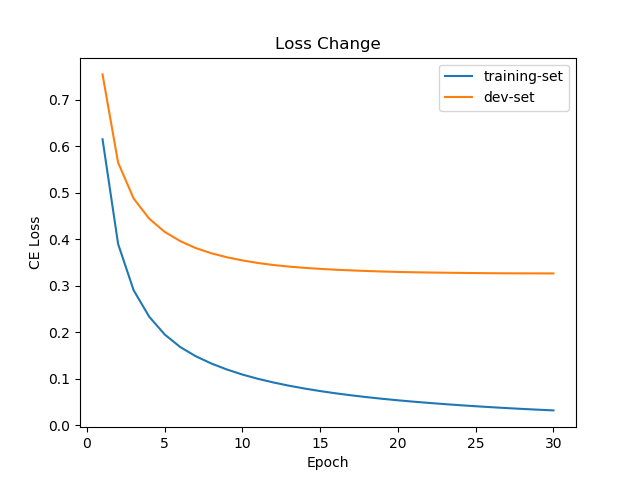
\includegraphics[width=2.5in]{Q1/loss_v1.png}
            \end{minipage}%
            \begin{minipage}[h]{0.5\linewidth}
                \centering
                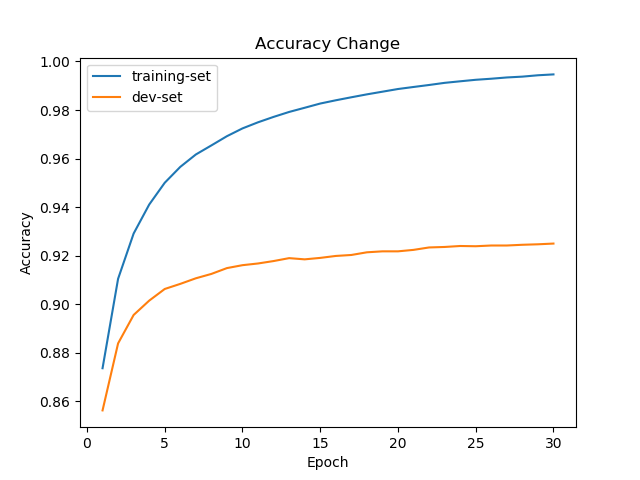
\includegraphics[width=2.5in]{Q1/acc_v1.png}
            \end{minipage}
        \end{figure}
        \item Training the BP neural network version 2 with regularization ($\lambda = 0.25$).
        \begin{figure}[h]
            \begin{minipage}[h]{0.5\linewidth}
                \centering
                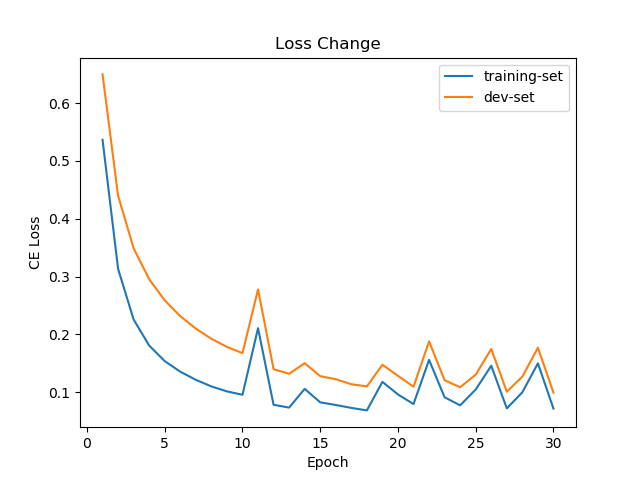
\includegraphics[width=2.5in]{Q1/loss_v2.png}
            \end{minipage}%
            \begin{minipage}[h]{0.5\linewidth}
                \centering
                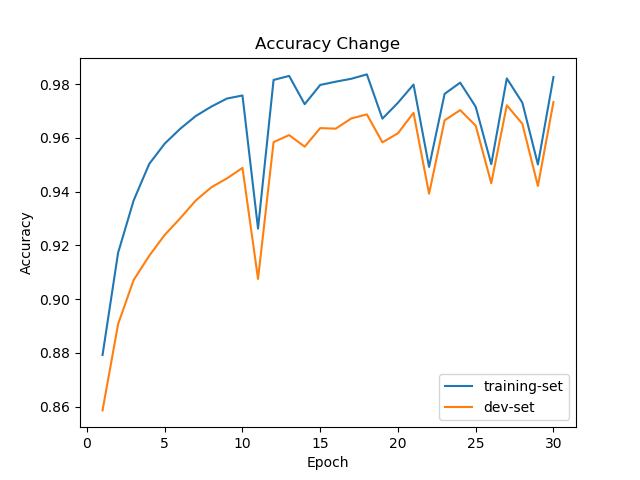
\includegraphics[width=2.5in]{Q1/acc_v2.png}
            \end{minipage}
        \end{figure}
        From the result we can see, with regularization of $W$, the overfitting is prevented but the training process has more fluctuation.
        \item The accuracy of test set is 0.928700 (without regularization) and 0.972300 (with regularization).
    \end{enumerate}

    \newpage
    \section*{EM Convergence }
    Since EM algorithm has converged, the lower bound of $l(\theta)$ is maxmized.
    Let LB represent the lower bound and we have (drop down some scripts for convenience)
    \begin{equation*}
        \begin{split}
            \bigtriangledown_\theta LB |_{\theta=\theta^*} &= \Sigma_i \Sigma_z Q_z \frac{Q_z}{p(x,z;\theta^*)}\frac{1}{Q_z} \bigtriangledown_\theta p(x,z;\theta) |_{\theta=\theta^*} \\
            &= \Sigma_i \Sigma_z \frac{\bigtriangledown_\theta p(x,z;\theta) |_{\theta=\theta^*}}{p(x;\theta^*)} \\
            &= \Sigma_i \frac{\bigtriangledown_\theta p(x;\theta) |_{\theta=\theta^*}}{p(x;\theta^*)} \\
            &= \Sigma_i \bigtriangledown_\theta [log p(x;\theta)]_{\theta=\theta^*} \\
            &= \bigtriangledown_\theta l(\theta) \\
            &= 0
        \end{split}
    \end{equation*}
    So when EM algorithm has converges, the $l(\theta)$ acheives the maxima.
    

    \section*{PCA}
    Since the line between projection and $x^{(i)}$ is perpendicular with the line between Origin point and projection, 
    minimizing the distance can be written:
    $$arg {min}_{\mu : \mu^T \mu=1 } \Sigma_{i=1}^m ||{x^{(i)}}^2-{x^{(i)}}^{T} \mu||_2$$
    Because ${x^{(i)}}^2$ is a constant, so the formula is equivalent to maxmizing the variance.


    \section*{Independent components analysis}
    The W matrix is as below shows:
   $$\left[ 
    \begin{matrix} 
    72.15081922&  28.62441682&  25.91040458& -17.2322227&  -21.191357 \\
    13.45886116 & 31.94398247&  -4.03003982& -24.0095722&   11.89906179\\
    18.89688784 & -7.80435173 & 28.71469558&  18.14356811& -21.17474522\\
    -6.0119837  & -4.15743607 & -1.01692289&  13.87321073&  -5.26252289\\
    -8.74061186 & 22.55821897&   9.61289023 & 14.73637074&  45.28841827\\
    \end{matrix}
    \right]$$
    The $S$ can be derived by $XW^T$.

    \newpage
    \section*{Markov decision processes}
    \begin{enumerate}[label=(\alph*)]
        \item let $s^a = ||V_1-V_2||_\infty$ and  $s^b = ||B(V_1)-B(V_2)||_\infty$, thus when $s=s^a,s^b$ the two formulas get their maximas.
        With Bellman equation, we have: ( assume $B(V_1)<B(V_2)$ )
        \begin{equation*}
            \begin{split}
                ||B(V_1)-B(V_2)||_\infty &= \gamma (\Sigma_{s'} P_{s^a a^1}(s')V_1(s') - \Sigma_{s'} P_{s^a a^2}(s')V_2(s') ) \\
                &\leq \gamma (\Sigma_{s'} P_{s^a a^2}(s')V_1(s') - \Sigma_{s'} P_{s^a a^1}(s')V_2(s') ) \\
                &=\gamma \Sigma_{s'} P_{s^a a^2}(V_1(s') -V_2(s')) \\
                &\leq (V_1(s^b)-V_2(s^b))  \\
            \end{split}
        \end{equation*}
        \item Assume the two points are $V_1$ and $V_2$, so $||B(V_1)-B(V_2)||_\infty = ||V_1-V_2||_\infty \leq \gamma||V_1-V_2||_\infty$, 
        which can't be true because $\gamma < 1$.
    \end{enumerate}

    \section*{Reinforcement Learning: The inverted pendulum }
    Finish the code in \href{https://github.com/zyxue/stanford-cs229/blob/master/Problem-set-4/6-reinforcement-learning-the-inverted-pendulum/control.py}{control.py}
    and make 5 training trails to get an average of 158 failure times to get converged.
    \begin{figure}[h]
        \centering
        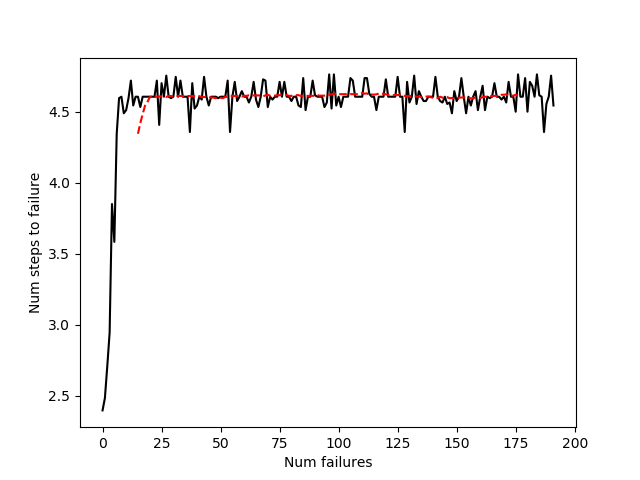
\includegraphics[width=0.8\textwidth]{Q6/192.png}
    \end{figure}
\end{document}